% evaluation description
\label{sec:eval}

We begin by evaluating our adaptation algorithm on a standard domain adaptation dataset.
We show that our algorithm is effectively able to adapt a deep CNN to a target domain with limited or no
labeled data.
Second, we will answer our question of whether or not using a high capacity 
model (deep CNN) in combination with a large labeled source dataset, will remove data set 
bias. 

%\et{Yangqing says something should go here, but Kate thinks the paragraph we had
%here before was repetitive, so TODO: come up with a non-repetitive paragraph to
%introduce this section}

%KS this was repetitive
%We now present experiments to evaluate the effectiveness of deep learned
%representations for domain adaptation. Using a subset of the
%ImageNet~\cite{ilsvrc2012} and Office~\cite{saenko-eccv10} datasets, we evaluate
%multi-class accuracy in a one-shot supervised domain adaptation setting where
%one labeled example of each target category is provided at adaptation time. We
%also evaluate the effectiveness of unsupervised adaptation methods, which use
%only the unlabeled test data in the target domain to perform adaptation.

\subsection{Datasets}
The Office~\cite{saenko-eccv10} dataset is a collection of images from three
distinct domains: Amazon, DSLR, and Webcam. The 31 categories in the dataset
consist of objects commonly encountered in office settings, such as keyboards,
file cabinets, and laptops. 

%Of these 31 categories, 16 overlap with the
%categories present in the 1000-category ImageNet classification task\footnote{
%The 16 overlapping categories are
%\textit{backpack},
% \textit{bike helmet},
% \textit{bottle},
% \textit{desk lamp},
% \textit{desktop computer},
% \textit{file cabinet},
% \textit{keyboard},
% \textit{laptop computer},
% \textit{mobile phone},
% \textit{mouse},
% \textit{printer},
% \textit{projector},
% \textit{ring binder},
% \textit{ruler},
% \textit{speaker},
% and
% \textit{trash can}.
%}.
ImageNet~\cite{ilsvrc2012} is the largest available dataset of image category labels. We use 1000 categories' worth of data (1.2M images) to train the network, and use the 31 categories that overlap with Office (approximately 1200 examples per category or  $\approx$37K images total) as labeled source classifier data.


\subsection{Experimental Setup \& Baselines}

 Each method is evaluated across 20 random train/test splits, and we report averages and standard errors for each setting. 
For each random train/test split we choose either one or three target training examples per category (as indicated) and use the rest for training.  The unsupervised adaptation methods operate in a transductive setting, so the target subspaces are learned from the unlabeled test data.

In all experiments, we use the fully trained deep CNN model described in Section~\ref{sec:decaf}, and extract feature representations from the three different fully connected layers of the CNN. We then compute the A-distance between the source and target data at each layer and choose to adapt at the layer with the lower A-distance. We then train a source classifier using these features on one of two source domains and adapt to the target domain. For all of our experiments, the highest network layer ended up producing the lowest A-distance.
This confirms our intuition that the higher layers have greater semantic invariance, and thus greater domain invariance. Thus, all of our experiments use that layer for adaptation.
In Section~\ref{sec:analysis} we also experimentally verify that the final eighth layer does indeed yield the best adaptation performance in this setting.
However, we expect that a lower layer may produce a lower A-distance for a more complex target domain scenario than that found in the benchmark Office dataset.

%The source domains we consider are either the Amazon domain, or the corresponding 16-category ImageNet subset where each category has many more examples.
%We focus on the Webcam domain as our target (test) domain, as Amazon-to-Webcam  was shown to be the only challenging shift in \cite{deeplearning-arxiv-2013} (the DSLR domain is much more similar to Webcam and did not require adaptation when using deep mid-level features). This combination exemplifies the shift from online web images to real-world images taken in typical office/home environments.
%Note that, regardless of the source domain chosen to learn the classifier, ImageNet data from all 1000 categories was used to train the network. 

%In addition, for the supervised adaptation setting we assume access to only a single example per category from the target domain (Webcam). 

%\ks{is this right? is this the standard test set?}




%\paragraph{Non-adaptive Baselines}
%In addition to the adaptation methods outlined in Section~\ref{sec:adapt-algs},
%we also evaluate using the following non-adaptive baselines.

%\begin{itemize}
%  \item{\textbf{SVM (source only)}: A support vector machine trained only on
%    source data. 
%\ks{why not the CNN itself, in case of imagenet? why re-train and SVM?}
%}
%  \item{\textbf{SVM (target only)}: A support vector machine trained only on
%    target data.}
%  \item{\textbf{SVM (source and target)}: A support vector machine trained on
%  both source and target data. To account for the large discrepancy between the
%  number of training data points in the source and target domains, we weighted
%  the data points such that the constraints from the source and target domains
%  effectively contribute equally to the optimization problem.  Specifically,
%  each source data point receives a weight of $\frac{n_t}{n_s+n_t}$, and each target
%  data point receives a weight of $\frac{n_s}{n_s+n_t}$, where $n_s,n_t$ denote the
%  number of data points in the source and target, respectively.}
%\end{itemize}

%Many of the adaptation methods we evaluate have hyperparameters that must be
%cross-validated for use in practice, so we set the parameters of the adaptation
%techniques as follows.

%First, the C value used for C-SVM in the classifier for all methods is set to $C=1$. Without any validation data we are not able to tune this parameter properly, so we choose to leave it as the default value. Since all methods we report require setting of this parameter, we feel that the relative comparisons between methods is sound even if the absolute numbers could be improved with a new setting for C.
%\begin{itemize}
  %\item{
  For the supervised early fusion adaptation method, which looks at the source and target data
  simultaneously, we weight 
  the data points such that the constraints from the source and target domains
 effectively contribute equally to the optimization problem.  Specifically,
  each source data point receives a weight of $\frac{n_t}{n_s+n_t}$, and each target
  data point receives a weight of $\frac{n_s}{n_s+n_t}$, where $n_s,n_t$ denote the
  number of data points in the source and target, respectively.
  %}
  %\item{
  
  For late fusion adaptation, we use the linear interpolation combination averaged over hyper parameter settings. We show the effect of changing this hyper parameter in Figure~\ref{fig:linint-eval} to help understand how performance varies as we trade off emphasis between the learned classifiers from the source and target domains. 
  %Again, we do not have the validation data to tune this parameter so we report in the tables the performance averaged across parameter settings. The plot vs $\alpha$ indicates that there is usually a best parameter setting that could be learned with more available data.
  %}
  %\item{
  %For PMT, we choose $\Gamma=1000$, which corresponds to allowing a large amount of transfer from the source classifier to the target classifier. We do this because the source-only classifier is
  %stronger than the target-only classifier (with ImageNet source). 
  %}
  %\item{
  For the unsupervised early fusion method we must choose a subspace dimension to project the data onto. We evaluated a variety of
  subspace dimensionalities and Figure~\ref{fig:sagfk-eval} shows that the overall method performance does not vary significantly with the dimensionality choice.
  %}
%\end{itemize}

\subsection{Full \emph{Office} Dataset Domain Adaptation Experiment}
In our experiments using the full Office dataset (31 categories),
we follow the standard training protocol for this dataset of using 20 source
examples per category~\cite{saenko-eccv10,gong-cvpr12}
 for the Amazon source domain and 8 images per category for Webcam or
 Dslr as the source domains. For the supervised adaptation setting 
 we assume 3 labeled target examples per category.


We begin by evaluating our framework and adaptation algorithm on the standard \emph{Office} dataset benchmark
for both supervised and unsupervised adaptation. We compare in both scenarios against four recently published methods.
We report our results on all 6 domain shifts possible with the 3 domains. Each of the previous methods only reported for the 3/6 possible shifts. 

The supervised adaptation setting results are shown in Table~\ref{table:full-semi} and the unsupervised adaptation results are shown in Table~\ref{table:full-unsuper}. We notice that our algorithm dramatically outperforms most of the competing methods with the exception of DLID on the webcam to dlsr shift in the supervised setting. These domains are very similar (only a resolution and lighting shift) and so would likely benefit from an adaptation approach that favors the source domain more than our weighting scheme does. 

\begin{table*}
  \setlength{\tabcolsep}{4pt}
  \small
\centering
\begin{tabular}{lcccccc}
\toprule
                     & $A \rightarrow D$   & $A \rightarrow W$   & $D \rightarrow A$   & $D \rightarrow W$   & $W \rightarrow A$   & $W \rightarrow D$   \\
\midrule
GFK(PLS,PCA)~\cite{gong-cvpr12} & - & 46.4$\pm$0.5 & - & 61.3$\pm$0.4 & - & 66.3$\pm$0.4\\
SA~\cite{fernando-iccv13} & - & 45.0 & - & 64.8 & - & 69.9\\
DLID~\cite{ref:dlid} & - & 51.9 & - & 78.2 & - & \bf{89.9}\\     
DA-NBNN~\cite{da-nbnn} & - & 52.8$\pm$3.7 & - & 76.6$\pm$1.7 &           - & 76.2$\pm$2.5\\
\midrule
 Ours (source only)   & $50.2 \pm 0.6$     & $45.6 \pm 0.5$     & $45.3 \pm 0.3$     & $\bm{86.5 \pm 0.3}$     & $44.2 \pm 0.3$     & $88.0 \pm 0.4$     \\
 Ours (target only)   & $77.4 \pm 0.5$     & $75.8 \pm 0.5$     & $55.6 \pm 0.5$     & $76.2 \pm 0.4$     & $55.9 \pm 0.4$     & $77.6 \pm 0.4$     \\
Ours (early fusion)& $\bm{78.5 \pm 0.5}$     & $\bm{77.4 \pm 0.4}$     & $\bm{58.4 \pm 0.5}$     & $85.2 \pm 0.3$     & $\bm{59.1 \pm 0.4}$     & $87.0 \pm 0.4$     \\
Ours (late fusion)& $69.3 \pm 0.8$ & $66.8 \pm 0.7$ & $56.7 \pm 0.4$ & $86.4 \pm 0.4$ & $56.3 \pm 0.6$ & $87.1 \pm 0.6$ \\
\bottomrule
\end{tabular}

\caption{Multi-class accuracy evaluation on the standard supervised adaptation setting with the \emph{Office} dataset. We evaluate on all 31 categories using the standard experimental protocol from ~\cite{saenko-eccv10}. Here, we compare against four state of the art domain adaptation methods (they all reported on only 3/6 domain shifts).}
\label{table:full-semi}
\end{table*}



\begin{table*}
  \setlength{\tabcolsep}{4pt}
  \small
\centering
\begin{tabular}{lcccccc}
\toprule
                     & $A \rightarrow D$   & $A \rightarrow W$   & $D \rightarrow A$   & $D \rightarrow W$   & $W \rightarrow A$   & $W \rightarrow D$   \\
\midrule
GFK(PLS,PCA)~\cite{gong-cvpr12} & - & 15.0$\pm$0.4 & - & 44.6$\pm$0.3 & - & 49.7$\pm$0.5\\
SA~\cite{fernando-iccv13} & - & 15.3 & - & 50.1& - & 56.9\\
DA-NBNN~\cite{da-nbnn} & - & 23.3$\pm$2.7 & - & 67.2$\pm$1.9 & - & 67.4$\pm$3.0\\
DLID~\cite{ref:dlid} & - & 26.1 & - & 68.9 & - & 84.9\\
\midrule
 Ours (source only)   & $\bm{50.2 \pm 0.6}$     & $45.6 \pm 0.5$     & $45.3 \pm 0.3$     & $\bm{86.5 \pm 0.3}$     & $\bm{44.2 \pm 0.3}$     & $\bm{88.0 \pm 0.4}$     \\
Ours (early fusion)   & $50.1 \pm 0.4$     & $\bm{46.6 \pm 0.7}$     & $\bm{45.5 \pm 0.4}$     & $86.2 \pm 0.3$     & $43.0 \pm 0.4$     & $86.7 \pm 0.5$     \\
\bottomrule
\end{tabular}

\caption{Multi-class accuracy evaluation on the standard unsupervised adaptation setting with the \emph{Office} dataset. We evaluate on all 31 categories using the standard experimental protocol from ~\cite{gong-cvpr12}. Here, we compare against four state of the art domain adaptation methods.(All methods reported on only 3/6 of the domain shifts).}
\label{table:full-unsuper}
\end{table*}



The distinct improvement of our method demonstrates that we are successfully able to transfer the supervised pre-trained deep CNN parameters to a target domain. However the question still follows, did we effectively remove bias and hence the need for our adaptation layer altogether? We address this question in our next experiment.

%\subsection{Effect of a High Complexity Model}

%\begin{table*}
\centering
\begin{tabular}{lcc}
\toprule
Adaptation Method & Training Data & Test Accuracy \\
\midrule
SVM (source only) & Amazon & $53.23 \pm 1.6$ \\
\midrule
GFK \cite{gong-cvpr12} & Amazon & $54.56 \pm 1.2$ \\
SA \cite{sa} & Amazon & $55.98 \pm 1.0$ \\
\bottomrule
\end{tabular}
%\caption{Adapting from a pre-trained ImageNet classifier to a new task label set.\jh{fix this caption}}

\caption{Amazon$\rightarrow$Webcam unsupervised adaptation experiments using
  DeCAF$_8$. In this setup, the labeled source data and the unlabeled target
  test data are available during training.}
\label{tab:amazon_fc8_unsup}
\end{table*}

%\begin{table*}
\centering
\begin{tabular}{lcc}
\toprule
Adaptation Method & Training Data & Test Accuracy \\
\midrule
SVM (source only) & Amazon & $53.23 \pm 1.6$ \\
SVM (target only) & Webcam & $63.13 \pm 1.9$ \\
\midrule
SVM (source and target) & Amazon+Webcam & $63.20 \pm 1.7$ \\
Late Fusion (Max) & Amazon+Webcam & $62.25 \pm 0.8$ \\
Late Fusion (LinInt Avg) & Amazon+Webcam & $64.56 \pm 1.3$ \\
\daume \cite{daume} & Amazon+Webcam & $70.51 \pm 1.7$ \\
PMT \cite{aytar-iccv11} & Amazon+Webcam & $66.77 \pm 2.1$ \\
MMDT \cite{hoffman-iclr13} & Amazon+Webcam & $66.23 \pm 1.4$ \\
\midrule
Late Fusion (Lin. Int. Oracle) & Amazon+Webcam & $71.49 \pm 1.3$ \\
\bottomrule
\end{tabular}
%\caption{Adapting from a pre-trained ImageNet classifier to a new task label set.\jh{fix this caption}}
\caption{Amazon$\rightarrow$Webcam supervised adaptation experiments using
  DeCAF$_8$. In this setup, the labeled source data and 1 additional labeled
  target example are available during training.}
\label{tab:amazon_fc8_sup}
\end{table*}


%We begin by evaluating the effect that a high complexity model (in this case, a
%fully trained convolutional net) has on mitigating domain shift.

%We evaluate using Amazon as a source domain. 
%Preliminary results on this setting are reported in~\cite{deeplearning-arxiv-2013}, but here 
%we extend the comparison here by
%presenting the results with more adaptation algorithms and more complete
%evaluation of hyperparameter settings. Tables~\ref{tab:amazon_fc8_unsup} and \ref{tab:amazon_fc8_sup} present % TODO fix reference
%multiclass accuracies for each algorithm using layer 8 from the deep
%network, which corresponds to the output from the final fully connected layer.

%\et{this paragraph needs to be redone with fc8.} An SVM trained using only Amazon data achieves 78.6\% in-domain accuracy (tested on the same domain) when using the DeCAF$_6$ feature and 80.2\% in-domain accuracy when using the DeCAF$_7$ feature. These numbers are significantly higher than the performance of the same classifier on Webcam test data, indicating that even with the DeCAF features, there is a still a domain shift between the Amazon and Webcam datasets. 
%This agrees with a similar result previously shown by Donahue et al.~\cite{deeplearning-arxiv-2013}.

%Next, we consider an unsupervised adaptation setting where no labeled examples are available from the target dataset. In this scenario, we apply two state-of-the-art unsupervised adaptation methods, GFK~\cite{gong-cvpr12} and SA~\cite{sa}. 
%Both of these methods make use of a subspace dimensionality hyperparameter.
%We show the results using a 100-dimensional subspace in Table~\ref{tab:amazon_fc8_unsup} and leave the discussion of setting this parameter until Section~\ref{sec:analysis}.

%We finally assume that a single example per category is available in the target domain.
%As Table~\ref{tab:amazon_fc8_sup} shows, supervised adaptation algorithms are able to provide significant improvement, even in the one-shot scenario. % TODO: fix reference



%For the purposes of comparison to prior work, we also ran a set of experiments
%using the standard evaluation protocol for the office dataset. \et{Gotta explain what
%the typical protocol is.} Results from these experiments can be seen in
%Table~\ref{tab:full_office}.

%\et{There will be an analysis of the results here once these experiments have
%been run.}

\subsection{Adapting with a Large Scale Source Domain}

\begin{figure}[h]
  \begin{center}
  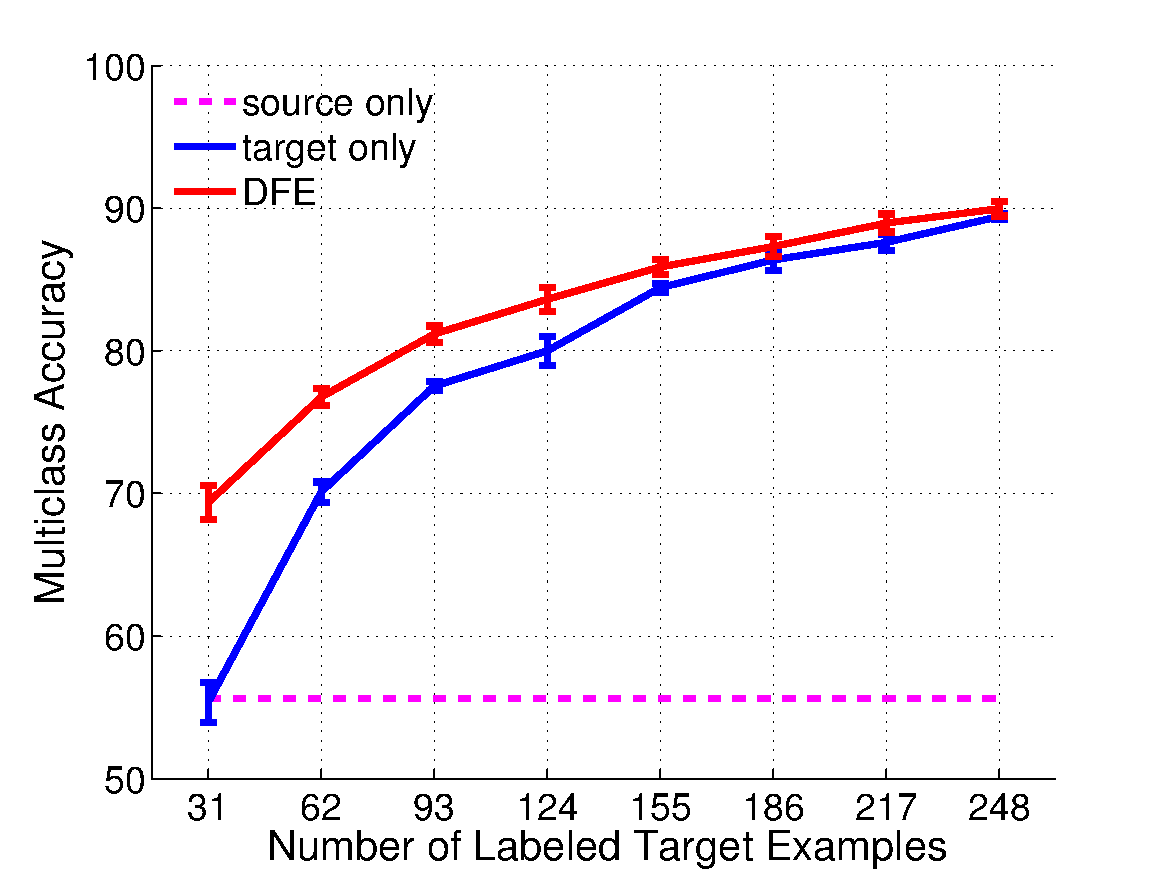
\includegraphics[width=.48\textwidth]{figs/imagenet_webcam_vary_num_target_examples}
  \end{center}
  \caption{Multiclass accuracy evaluation on the Imagenet to Webcam shift while varying the number of labeled target examples. DFE stays significantly ahead of the non-adaptive baseline until 5 labeled target examples per category are available (155 labeled examples total).}
  \label{fig:vary_num_target}
\end{figure}

We now address one of the main questions of this paper: Is there still a domain shift when using a large source dataset such as ImageNet? To begin to answer this question we follow mostly the same experimental paradigm as the previous experiment, with the only differences being that we use 5 train/test splits instead of 20, and we use ImageNet as our source dataset.
We investigate using the webcam domain as our target since it is the most distinct from ImageNet. 
Additionally, we only use one labeled target example for the supervised adaptation experiment. We do this to determine how useful a labeled target example is during adaptation. If there is very little bias between ImageNet and the webcam domain, then a single target example would not provide much adaptation benefit.
The results for unsupervised adaptation are shown in Table~\ref{tab:imagenet_fc8}(a), and the results for supervised adaptation are shown in Table~\ref{tab:imagenet_fc8}(b). % TODO fix reference
\begin{table*}
\begin{tabular}{c c}
\begin{tabular}{lcc}
\toprule
Adaptation Method & Test Accuracy \\
\midrule
source only & $66.23 \pm 0.8$ \\
\midrule
Early Fusion  & $66.08 \pm 1.1$ \\
\bottomrule
\end{tabular}

&
\hspace{1cm}
\begin{tabular}{lcc}
\toprule
Adaptation Method & Test Accuracy \\
\midrule
source only  & $66.23 \pm 0.8$ \\
target only  & $63.13 \pm 1.9$ \\
\midrule
Late Fusion & $70.56 \pm 1.2$ \\
Early Fusion & {$\bm{77.15 \pm 1.1}$} \\
\bottomrule
\end{tabular}
\\ & \\
(a) Unsupervised Adaptation & (b) Semi-Supervised Adaptation

\end{tabular}
%\caption{Adapting from a pre-trained ImageNet classifier to a new task label set.\jh{fix this caption}}
\caption{Imagenet$\rightarrow$Webcam adaptation experiments. In this setup, the labeled source data and the unlabeled target
  test data are available during training in both scenarios.}
\label{tab:imagenet_fc8}
\end{table*}

%\begin{table*}
\centering
\begin{tabular}{lcc}
\toprule
Adaptation Method & Training Data & Test Accuracy \\
\midrule
SVM (source only) & Imagenet & $66.23 \pm 0.8$ \\
SVM (target only) & Webcam & $63.13 \pm 1.9$ \\
\midrule
SVM (source and target) & Imagenet+Webcam & $75.13 \pm 1.1$ \\
Late Fusion (Max) & Imagenet+Webcam & $71.77 \pm 1.4$ \\
Late Fusion (LinInt Avg) & Imagenet+Webcam & $70.56 \pm 1.2$ \\
\daume \cite{daume} & Imagenet+Webcam & \textcolor{red}{$\bm{77.15 \pm 1.1}$} \\
PMT \cite{aytar-iccv11} & Imagenet+Webcam & $70.28 \pm 1.8$ \\
MMDT \cite{hoffman-iclr13} & Imagenet+Webcam & $73.96 \pm 1.2$ \\
\midrule
Late Fusion (Lin. Int. Oracle) & Imagenet+Webcam & {$\bm{76.61 \pm 1.5}$} \\
\bottomrule
\end{tabular}
%\caption{Adapting from a pre-trained ImageNet classifier to a new task label set.\jh{fix this caption}}
\caption{Imagenet$\rightarrow$Webcam supervised adaptation experiments using
  DeCAF$_8$. In this setup, the labeled source data and 1 additional labeled
  target example are available during training.}
\label{tab:imagenet_fc8_sup}
\end{table*}


Interestingly, we find that we are not able to adapt in the unsupervised scenario, however, even with a single labeled target example per category (31 images total!), we are able to produce a dramatic performance boost -- 56\% up to 70\% multi class accuracy.

We also investigate how performance varies as we allow ourselves access to more labeled data in the target domain. We plot performance of both the target only baseline and DFE as we vary the number of labeled target examples in Figure~\ref{fig:vary_num_target}.
As the results indicate, DFE provides a significant edge over the simple non-adaptive baseline for 4 or fewer labeled examples in the target domain. Thus, even when we do not limit ourselves to the extreme setting of only one labeled target example, using DFE continues to be effective. For a more complex target domain the benefit would likely continue with even more target examples.

% \ks{this paragraph is easy to lose.. isn't this the main point of the paper?}
%\et{This paragraph also needs to be redone with FC8.}
%Again, we first verify that the source only SVM achieves higher performance when tested on in-domain data than on Webcam data. 
%Indeed, for the 16 overlapping labels, the source SVM produces 62.50\% accuracy on ImageNet data using DeCAF$_6$ features and 74.50\% accuracy when using DeCAF$_7$ features. 
%Compare this to the 54\% and 59\% for Webcam evaluation and a dataset bias is still clearly evident.

 

%In addition, unsupervised adaptation approaches are more effective than for the smaller source domain experiment. 

\et{I left the following paragraph kind of vague. Is this a problem?}

We also attempted to fine tune the CNN on the target training data as another
baseline to compare against. However, even with 3 labeled target examples per
category, as is the standard for the Office dataset, we were unable to improve
performance beyond the non-adaptive target only baseline, despite trying many
variations of fine-tuning. It appears that 93 labeled images is simply not
enough data to fine-tune a CNN of this size.

\subsection{Analysis and Practical Considerations}
\label{sec:analysis}
\input analysis


\input linint-fig
